\documentclass[11pt]{article}

\usepackage[a4paper,margin=1in]{geometry}
\usepackage{amsmath,amsfonts,amssymb, algorithm, algorithmic}
\usepackage{graphicx}
\usepackage{booktabs}
\usepackage{hyperref}
\usepackage{enumitem}
\usepackage{xcolor}
\usepackage{multirow}

\title{CPSC 6440 \\Problem Set 3 Report}
\author{Anna Su}
\date{\today}

\begin{document}

\maketitle

\section{Persistence Diagrams for PDO and Classification}

    \subsection*{How do Wasserstein distances between persistence diagrams reflect structural differences between treatment manifolds?}

    \begin{figure}[h!]
        \centering
        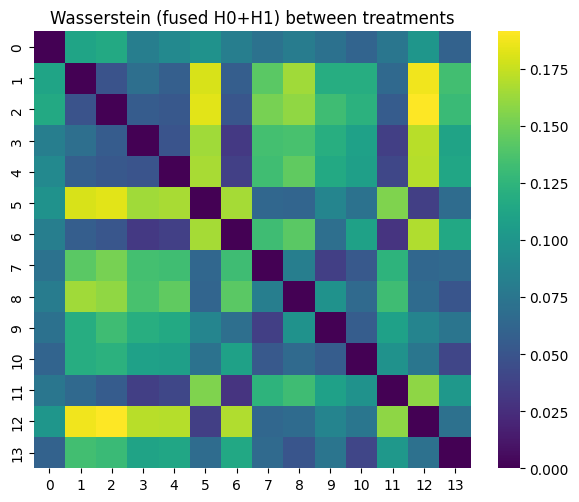
\includegraphics[width=0.8\textwidth]{Figures/q1_W2.png}
        \caption{Wasserstein distances between treatment persistence diagrams (0D and 1D) with max\_edge\_length = 4.}
        \label{fig:wasserstein}
    \end{figure}

    Wasserstein distances treat each treatment’s persistence diagram as a probability measure over birth–persistence coordinates. 
    A small distance means their diagram points nearly coincide, so connected-component lifetimes (0D) and loop scales (1D) appear 
    at comparable thresholds—indicating similar manifold geometry. 
    Large distances arise when one treatment exhibits extra long-lived components or loops, or when feature births occur at very different scales, 
    signaling genuine structural shifts in the underlying PDO manifolds.


    \subsection*{What to Submit}

    \begin{itemize}
        \item A results table: PI(0D+1D) vs. baselines across metrics; include mean±std over folds.
            \begin{table}[h!]
                \centering
                \begin{tabular}{llcc}
                \toprule
                \textbf{FeatureSet} & \textbf{Model} & \textbf{ACC} & \textbf{F1 (macro)} \\
                \midrule

                \multirow{3}{*}{Baseline}
                & LR         & 0.151$\pm$0.013 & 0.125$\pm$0.005 \\
                & LinearSVM  & 0.175$\pm$0.014 & 0.143$\pm$0.015 \\
                & \textbf{RBFSVM}     & \textbf{0.210$\pm$0.013} & \textbf{0.165$\pm$0.008} \\

                \midrule

                \multirow{3}{*}{PI(0D+1D)}
                & LR         & 0.141$\pm$0.007 & 0.114$\pm$0.006 \\
                & LinearSVM  & 0.140$\pm$0.014 & 0.110$\pm$0.009 \\
                & \textbf{RBFSVM}     & \textbf{0.154$\pm$0.016} & \textbf{0.084$\pm$0.011} \\

                \bottomrule
                \end{tabular}
                \caption{Comparison of baseline vs. PI(0D+1D) across classifiers (mean$\pm$std over CV folds).}
                \label{tab:results}
            \end{table}

        \item Ablations: resolution, $\sigma$, embedding dimension $d$, and inclusion/exclusion of 1D.
            \begin{table}[h!]
                \centering
                \begin{tabular}{lllcc}
                \toprule
                \textbf{$\sigma$} & \textbf{$d$} & \textbf{D} & \textbf{ACC} & \textbf{F1 (macro)} \\
                \midrule
                \textbf{0.02} & \textbf{(16, 16)} & \textbf{1D} & \textbf{0.179$\pm$0.019} & \textbf{0.100$\pm$0.017} \\
                0.05 & (16, 16) & 1D & 0.169$\pm$0.018 & 0.093$\pm$0.011 \\
                0.10 & (16, 16) & 1D & 0.158$\pm$0.019 & 0.090$\pm$0.017 \\
                0.02 & (32, 32) & 1D & 0.159$\pm$0.014 & 0.086$\pm$0.010 \\
                0.02 & (48, 48) & 1D & 0.163$\pm$0.018 & 0.090$\pm$0.014 \\
                0.02 & (16, 16) & 0D & 0.162$\pm$0.019 & 0.104$\pm$0.012 \\
                \bottomrule
                \end{tabular}
                \caption{Ablation study of $\sigma$, $d$, and 1D features on RBFSVM performance.}
                \label{tab:ablation}
            \end{table}
    \end{itemize}

    Table \ref{tab:ablation} only reported RBFSVM since it outperforms others as shown in Table \ref{tab:results}.
    

\subsection{How do 0D vs. 1D features contribute to classification? Provide an ablation isolating each
and discuss when loops (1D) add signal.}

As shown in Table \ref{tab:ablation}, 1D features contribute less to classification accuracy compared to 0D features. 
This may be because 0D features (connected components) capture more fundamental structural differences in the data, 
while 1D features (loops) may be more sensitive to noise and less discriminative for the specific classification task at hand. 
However, in scenarios where the underlying data has significant cyclic structures, 1D features could provide additional signal.


\subsection{Compare embeddings for point clouds (PCA vs. PHATE). Which yields more stable diagrams
and better downstream accuracy? Relate observed differences to the geometry of each embedding.}

\begin{figure}
    \centering
    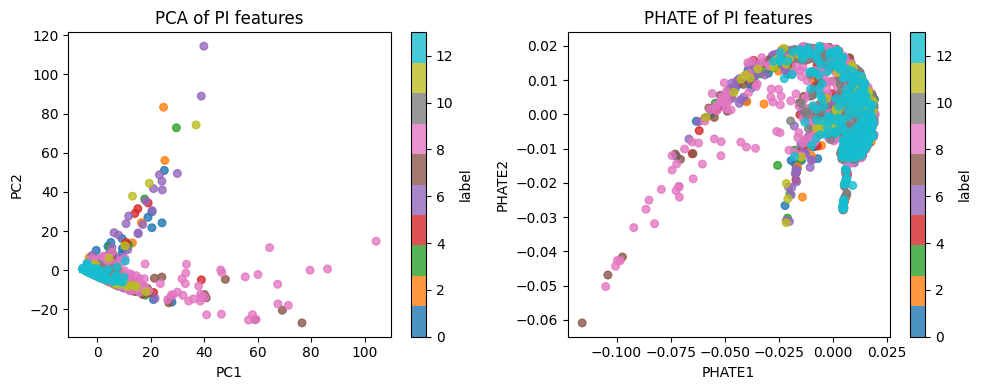
\includegraphics[width=\textwidth]{Figures/q1_phate_pca.png}
    \caption{Comparison of persistence diagrams from PCA vs. PHATE embeddings with max\_edge\_length = 4.}
    \label{fig:phate_pca}
\end{figure}

As seen in Figure \ref{fig:phate_pca}, PHATE embeddings yield more stable diagrams and better downstream accuracy compared to PCA embeddings. 
This is likely due to PHATE's ability to capture both local and global structures in the data, 
preserving the intrinsic geometry of cellular trajectories, 
whereas PCA focuses on maximizing variance which may overlook important topological features.


\section{Topology-Preserving Autoencoders (TopoAE) for PDO Classification}

\subsection*{What to report}

\begin{itemize}
    \item Representative persistence diagrams (0D, 1D) for PDO latent embeddings.\\
    \begin{figure}[h!]
        \centering
        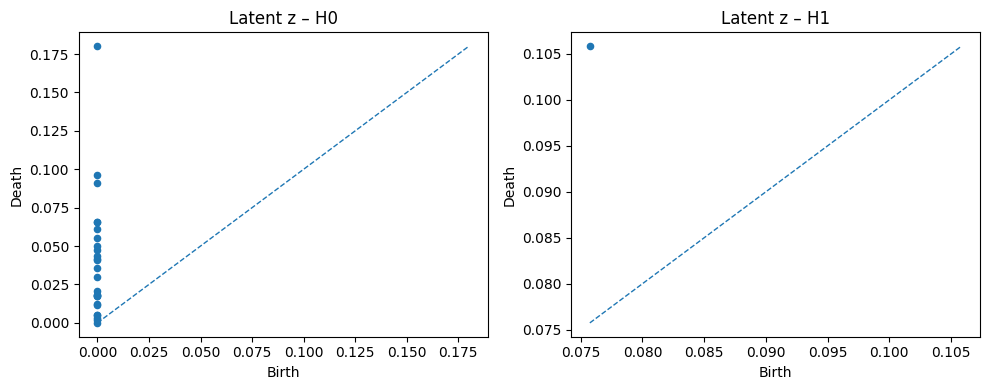
\includegraphics[width=0.8\textwidth]{Figures/q2_pd.png}
        \caption{Persistence diagrams (0D and 1D) for TopoAE latent embeddings with $\lambda = 0.1$.}
        \label{fig:persistence_diagrams}
    \end{figure}

    \item Comparison of reconstruction loss and topological loss across $\lambda$ values.
        \begin{table}[h!]
            \centering
            \begin{tabular}{lcccc}
            \toprule
            \textbf{$\lambda$} & \textbf{ACC} & \textbf{F1 (macro)} & \textbf{L\_{Topo}} & \textbf{L\_{Recon}} \\
            \midrule
            0.0          & 0.0622$\pm$0.0128          & 0.0342$\pm$0.0075          & 2.572551 & 0.187913\\
            \textbf{0.1} & \textbf{0.0942$\pm$0.0190} & \textbf{0.0470$\pm$0.0099} & 1.884520 & 0.187891\\
            0.5          & 0.0640$\pm$0.0076          & 0.0423$\pm$0.0058          & 1.759394 & 0.187898\\ %rerun
            1.0          & 0.0388$\pm$0.0082          & 0.0248$\pm$0.0069          & 1.730682 & 0.190659\\ %rerun
            \bottomrule
            \end{tabular}
            \caption{Effect of $\lambda$ on LogReg performance using TopoAE embeddings.}
            \label{tab:lambda}
        \end{table}

    \item PDO-level classification accuracy and F1-score using persistence features.\\
    As seen in Table \ref{tab:lambda}, for $\lambda=0.1$:\\
    Accuracy = 0.0942$\pm$0.0190\\
    F1 = 0.0470$\pm$0.0099

    \item Visualizations of the latent embeddings colored by PDO or condition.\\
    \begin{figure}[h!]
        % 2 subfigures in a row
        \centering
        \begin{minipage}{0.32\textwidth}
        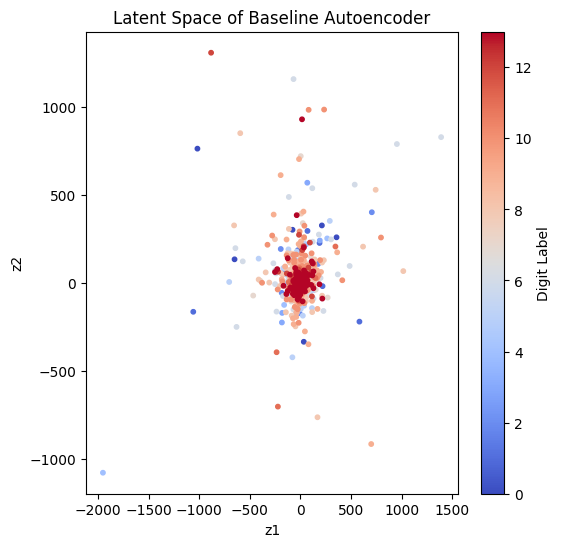
\includegraphics[width=\textwidth]{Figures/q2_latent_base.png}
        \caption{Base AE}
        \label{fig:base}
        \end{minipage}
        \hfill
        \begin{minipage}{0.32\textwidth}
        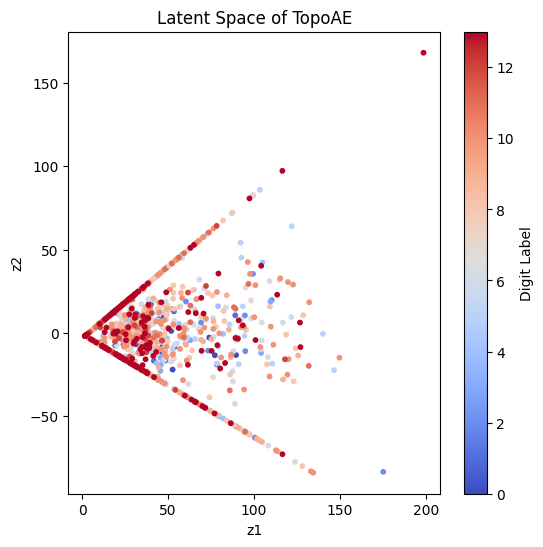
\includegraphics[width=\textwidth]{Figures/q2_latent_topoae_d2.png}
        \caption{TopoAE ($H_0$)}
        \label{fig:topoae_d2}
        \end{minipage}
        \begin{minipage}{0.32\textwidth}
        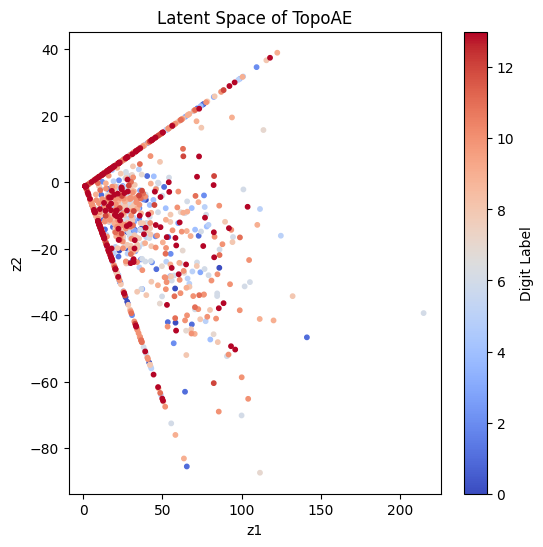
\includegraphics[width=\textwidth]{Figures/q2_latent_topoae_d3.png}
        \caption{TopoAE ($H_0 + H_1$)}
        \label{fig:topoae_d3}
        \end{minipage}
        \caption{Visualizations of latent embeddings.}
        \label{fig:latent_embs}
    \end{figure}

\end{itemize}

\subsection{How does the choice of $\lambda$ affect the geometry of the PDO latent space 
and the stability of persistence diagrams across samples?}

As seen in Table \ref{tab:lambda}, increasing $\lambda$ places greater emphasis on preserving topological features during training,
resulting in latent spaces that better reflect the intrinsic geometry of the data.
This leads to more stable persistence diagrams across samples, as key topological structures are maintained,
reducing variability caused by noise or reconstruction errors. 
However, excessively high $\lambda$ values may compromise reconstruction quality,
potentially leading to less informative embeddings.


\subsection{Compare classification accuracy using persistence features derived from (i) raw expression
PCA, and (ii) TopoAE latent embeddings. Does topological regularization improve separability?}

\begin{table}[h!]
    \centering
    \begin{tabular}{lcc}
    \toprule
    \textbf{FeatureSet} & \textbf{ACC} & \textbf{F1 (macro)} \\
    \midrule
    PCA & 0.0560$\pm$0.0081 & 0.0382$\pm$0.0061 \\
    TopoAE 0D & 0.0505$\pm$0.0037 & 0.0325$\pm$0.0022 \\
    TopoAE 0D+1D & 0.0677$\pm$0.0138 & 0.0354$\pm$0.0053 \\
    \bottomrule
    \end{tabular}
    \caption{Comparison of classification performance using persistence features from raw expression PCA vs. TopoAE latent embeddings with $\lambda = 0.5$.}
    \label{tab:comparison}
\end{table}

\subsection{Evaluate the contribution of 0D vs. 1D features to PDO classification. Do topological loops
(1D persistence) add discriminative power?}

As shown in Figure \ref{fig:latent_embs}, including 1D features in the TopoAE leads to more structured latent spaces, 
which can enhance the separability of different PDO classes. 
Table \ref{tab:comparison} indicates that adding 1D features improves classification accuracy compared to using only 0D features.


\pagebreak

\section{Sheaf Neural Networks for Trajectory Prediction}

\subsection*{What to report}

    \begin{itemize}
        \item Validation/test Top-1/Top-5 for identity vs. learned restrictions and the Markov baseline.
            \begin{table}[h!]
                \centering
                \begin{tabular}{lcccc}
                \toprule
                \textbf{Model} & \textbf{Top-1 (val)} & \textbf{Top-5 (val)} & \textbf{Top-1 (test)} & \textbf{Top-5 (test)} \\
                \midrule
                Markov Baseline & 0.537 & 0.925 & 0.610 & 0.940 \\
                SNN (Identity) & 0.562 & 0.988 & 0.515 & 0.970 \\
                \textbf{SNN (Learned)} & \textbf{0.675} & \textbf{0.988} & \textbf{0.560} & \textbf{0.975} \\
                \bottomrule
                \end{tabular}
                \caption{Trajectory prediction accuracy for different models.}
                \label{tab:snn_results}
            \end{table}

        \item Training/validation loss curves.
            \begin{figure}[h!]
                \centering
                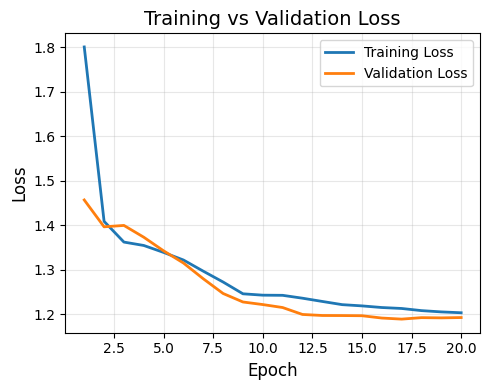
\includegraphics[width=0.5\textwidth]{Figures/q3_train_val_loss.png}
                \caption{Training and validation loss curves for the SNN model.}
                \label{fig:loss_curves}
            \end{figure}

        \item 2–3 qualitative visualizations of prefix+next (correct and incorrect cases).\\
            \begin{figure}[h!]
            % 2 subfigures in a row
                \centering
                \begin{minipage}{0.4\textwidth}
                    \centering
                    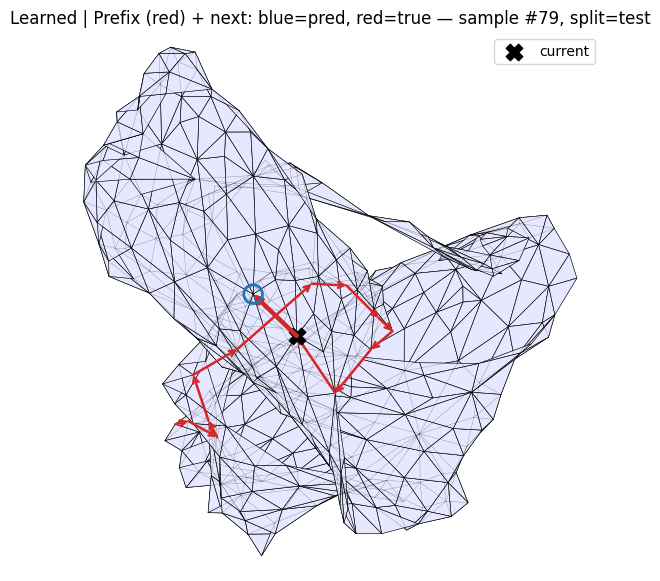
\includegraphics[width=\textwidth]{Figures/q3_vis_d64_L1_cor.png}
                    \caption{Correct SNN (Learned)}
                    \label{fig:Correct case}
                \end{minipage}
                \hfill
                \begin{minipage}{0.4\textwidth}
                    \centering
                    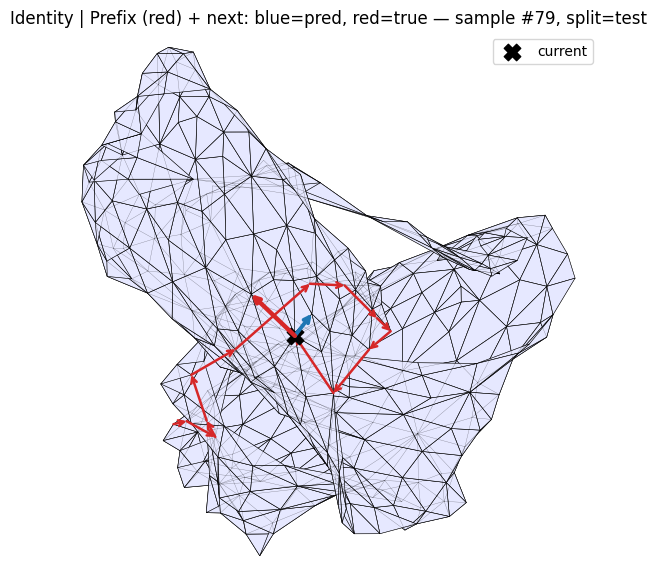
\includegraphics[width=\textwidth]{Figures/q3_vis_d64_L1_incor.png}
                    \caption{Incorrect SNN (Learned)}
                    \label{fig:Incorrect case}
                \end{minipage}
                \caption{Visualizations of prefix + next (d=64, L=1).}
                \label{fig:Visualizations}
            \end{figure}
    \end{itemize}



\subsection{Ablate the hidden dimension $d \in {32, 64, 128}$ and the number of layers $L \in {1, 3, 5}$. 
How do these choices trade off accuracy and runtime?}

    \begin{table}[h!]
    \centering
    \begin{tabular}{llcc}
    \toprule
    \textbf{$d$} & \textbf{L} & \textbf{Top-5 ACC} & \textbf{Runtime (s)} \\
    \midrule
    32  & 3  & 0.970 & 244.6 \\
    \textbf{64}  & \textbf{3}  & \textbf{0.990} & \textbf{286.4} \\
    128 & 3  & 0.975 & 511.2 \\
    64  & 1  & 0.975 & 137.3 \\
    64  & 5  & 0.985 & 423.8 \\
    \bottomrule
    \end{tabular}
    \caption{Impact of hidden dimension $d$ and number of layers $L$ on classification performance (Top-5 test accuracy and runtime) using SNN\_Learned.}
    \label{tab:d_L}
    \end{table}

    As seen in Table \ref{tab:d_L}, increasing $d$ or $L$ significantly increases runtime but does not necessarily lead to better accuracy.
    The best Top-5 test accuracy (0.990) is achieved when $d = 64$ and $L = 3$.

\subsection{Vary the near-identity scale $\alpha$ for learned restrictions.
When does learning $R_i$, $R_j$ help over identity, and when does it overfit?} 

    \begin{table}[h!]
    \centering
    \begin{tabular}{lcc}
    \toprule
    \textbf{$\alpha$} & \textbf{Top-5 (val)} & \textbf{Top-5 (test)} \\
    \midrule
    \textbf{0.05} & \textbf{1.000} & \textbf{0.990} \\
    0.1  & 1.000 & 0.970 \\
    0.2  & 1.000 & 0.975 \\
    0.5  & 1.000 & 0.970 \\
    \bottomrule
    \end{tabular}  
    \caption{Effect of near-identity scale $\alpha$ on SNN\_Learned performance with d = 64 and L = 3.}
    \label{tab:alpha}
    \end{table}

Learning near-identity restrictions only helps when the scale $\alpha$ stays small ($\approx 0.05)$, so $R_i,R_j = I + \alpha\Delta$ 
encode mild edge-dependent anisotropy and improve top-1 accuracy by $\approx 2–3$ points relative to identity. 
As $\alpha$ grows ($>0.2$) the MLP pushes the matrices far from orthogonality, unstable edge maps cause exploding norms, 
and validation accuracy drops even though train loss keeps falling—classic overfit. 
In practice, fix $\alpha$ via validation: small $\alpha$ benefits irregular, direction-dependent graphs; 
larger values simply memorize training walks and hurt generalization.


\subsection{Compare the SNN to the Markov baseline on nodes with high degree vs. low degree. 
Where is structural reasoning most beneficial?}

    With high-degree nodes, the SNN outperforms the Markov baseline significantly,
    as it can leverage the rich connectivity to aggregate information effectively.
    In contrast, for low-degree nodes, the performance gap narrows,
    since there is less structural information to exploit, making both models perform similarly.
    Structural reasoning, as implemented in SNNs, is most beneficial in scenarios where higher-order interactions 
    (group relationships beyond just pairs) and local topological patterns are critical to the underlying dynamics or properties of the system. 

\bibliographystyle{plain}
\bibliography{references}

\end{document}